\chapter{System Design}
The following chapter will explain the design process for the prototype for the project. The components of the project is broken into four parts: Machine Learning Algorithm on what algorithm and ML library was used, Data Preparation for insight into the data utilised, Training for explanation on the approach for training the model and Deployment for the process in which the model was deployed for production. Lastly, the overall system architecture will be explained.

////******* This will be later updated for the final design *******///

\section{Machine Learning Model}

For designing the model, the Keras machine learning library with the TensorFlow backend was used in order to easily create a convolutional neural network. The network consists of two convolution layers, two MaxPooling layers and a fully-connected layer. The model has two outputs nodes that provide classification of two emotions: happy or sad. The model used supervised learning, with labels for the images it was training on, which will be brought forward in the following section.\\

%Building a Convolutional Neural Network in Keras

\section{Data Preparation}
As stated by \citeauthor*{LOPES} that there is a scarcity of public datasets with for facial expression images, therefore a dataset was created for created by bulk downloading images from Google Images on searches such as "Happy Human face" and "Person Frowning". These images where split into a 30/70 split. The training data consisted of 70\% of the images and the remaining 30\% was used in testing. Within these these training and test sets are folders titles \textbf{happy} and \textbf{sad}. These folder names where used as labels during the training phase of the prototype.

\section{Training}

Due to insufficient hardware, the approach of cloud training was needed in order to train the model. The Python code and the dataset were pushed to a containerized TensorFlow environment on the FloydHub cloud platform. The output of the trained weights is saved to a \textit{.h5} file and the trained model is JSON file.

%pushing to floydhub
%saving the model to a h5 file

\section{Deployment}
In order to deploy the trained model to production, a Python API was developed using the Flask package, which provides many libraries to run python code on a server. The API is hosted on Heroku PaaS as they provide an easy-to-use and free basice tier service for hosting Python apps. The trained weights and model files are also deployed with the API. These are read in and initialised from their respective files when the API successfully build and deploys. The API accepts 'POST' requests and takes the image as input. The image is then fed into the model and a classification of \textbf{Happy} or \textbf{Sad} is made, this is then returns to the original sender.

Secondly, a Node.JS web app was developed in order to display how this model can be used in production. The application was also deployed to heroku. The application uses the clients webcam in order to record their face. This takes snapshots of the users face and sends the images to the Python API in two second intervals. The application then receives the response from the API and displays it to the screen in the format of \textit{'Emotion Detected: Happy'} for example. The web app is simple in design but more features will be added in the final implementation, which will be explained in the system architecture section.
%Creating the Survey App in node
%Creating a python API 


\section{Concluding Remarks of System Architecture Design}
Figure \ref{proto} illustrates a logical topology of final project. The primary component such as a web application that records the users face and the model deployment have already been achieved.\\

\begin{figure}[ht]
	\begin{center}
		\advance\leftskip-3cm
		\advance\rightskip-3cm
		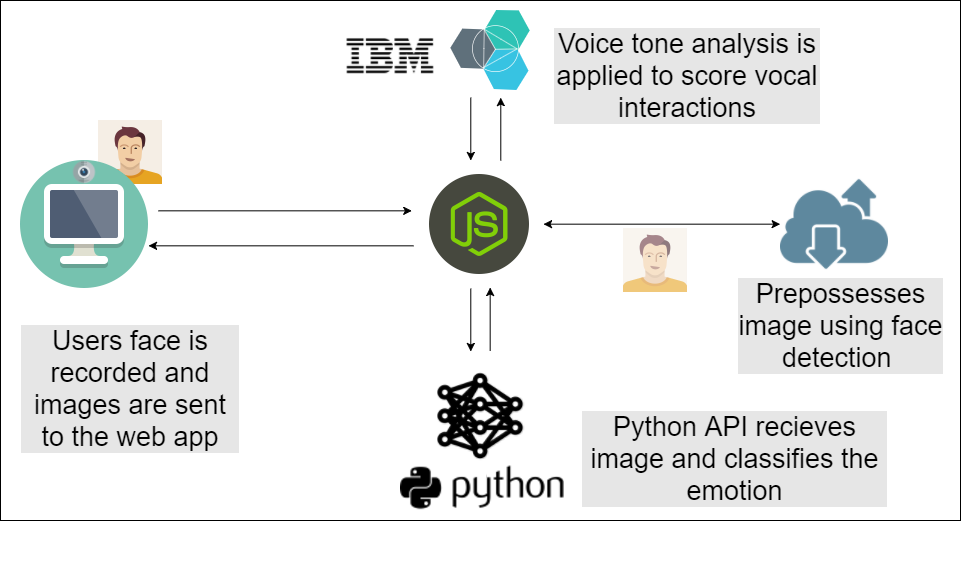
\includegraphics[keepaspectratio=true,scale=0.5]{__resources/arch.png}
		\caption{System architecture of the prototype}
		\label{proto}
	\end{center}
\end{figure}

However, further functionalities such as image preprocessing of the captured images is needed for more accurate classifications. Also, a tone analysis feature should be implemented to reach the over all goal of the project.
In conclusion, it can be noted that 1/2 of the project is achieved within this prototype.

